% Permission is granted to copy, distribute and/or modify this document
% under the terms of the GNU Free Documentation License, Version 1.2
% or any later version published by the Free Software Foundation;
% with no Invariant Sections, no Front-Cover Texts, and no Back-Cover
% Texts.  A copy of the license is included in the section entitled "GNU
% Free Documentation License".
% Copyright 2014 EDF
%

%%%%%%%%%%%%%%%%%%%%%%%%%%%%%%%%%%%%%%%%%%%%%%%%%%%%%%%%%%%%%%%%%%%%%%%%%%%%%%%%%%%%%%%%%%
\section{Architecture guide}

This document makes up the general specification design for the architecture of the OTPMML module.

\subsection{DAT}

\begin{figure}[htb]
  \begin{center}
    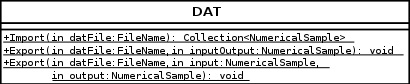
\includegraphics[scale=0.8]{DAT.png}
    \caption{DAT class}\label{fig:archi:DAT}
  \end{center}
\end{figure}

The \texttt{DAT} class is a utility class to import and export Uranie \texttt{.dat} files.  It contains only static methods.

\subsection{NeuralNetwork}

\begin{figure}[htb]
  \begin{center}
    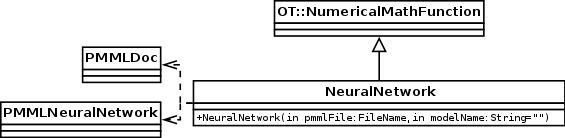
\includegraphics[scale=0.8]{NeuralNetwork.png}
    \caption{NeuralNetwork class}\label{fig:archi:NeuralNetwork}
  \end{center}
\end{figure}

The \texttt{NeuralNetwork} class inherits from \texttt{NumericalMathFunction}.
It uses \texttt{PMMLDoc} and \texttt{PMMLNeuralNetwork} internal classes to parse \texttt{.pmml} files written by Uranie.

\subsection{RegressionModel}

\begin{figure}[htb]
  \begin{center}
    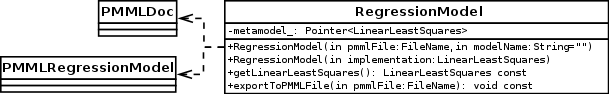
\includegraphics[scale=0.8]{RegressionModel.png}
    \caption{RegressionModel class}\label{fig:archi:RegressionModel}
  \end{center}
\end{figure}

The \texttt{RegressionModel} class is a wrapper around \texttt{RegressionModel} XML elements found in \texttt{.pmml} files.
It uses \texttt{PMMLDoc} and \texttt{PMMLRegressionModel} internal classes.

\subsection{PMML Internal Classes}

\subsubsection{PMMLDoc}

\begin{figure}[htb]
  \begin{center}
    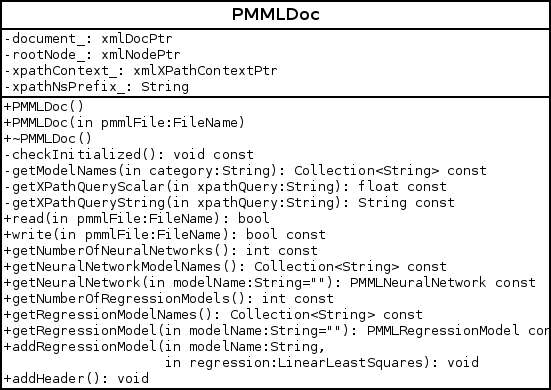
\includegraphics[scale=0.8]{PMMLDoc.png}
    \caption{PMMLDoc class}\label{fig:archi:PMMLDoc}
  \end{center}
\end{figure}

The \texttt{PMMLDoc} class reads an XML file (in the PMML 3.0 format, which is
the format used by Uranie), and provides several methods used by
\texttt{PMMLNeuralNetwork} and \texttt{PMMLRegressionModel} classes.
It internally uses LibXML2 library to handle XML data; this library must be initialized
before parsing XML data, and memory must be explicitly deallocated when its job is over.
For this reason, it had been decided to not expose \texttt{PMMLDoc} to the Python interface.
Calls to \texttt{xmlInitParser} and \texttt{xmlCleanupParser} are performed by higher-level
classes \texttt{NeuralNetwork} and \texttt{RegressionModel}.

XPath is used extensively to extract informations from XML data; two methods,
\texttt{getXPathQueryScalar} and \texttt{getXPathQueryString}, are provided for
simple usages.  \texttt{PMMLNeuralNetwork} and \texttt{PMMLRegressionModel} classes
are declared \texttt{friend} so that they can use these methods.

The \verb+xpathContext_+ member stores the current XPath context, and is modified by
\texttt{setXPathContext} methods of \texttt{PMMLNeuralNetwork} and \texttt{PMMLRegressionModel} classes
to point to their respective XML elements.

There are some caveats with XML namespaces when using XPath.  In order to parse XML files with or
without namespaces, an \verb+xpathNsPrefix_+ member has been added.

\paragraph{Note:}
In \texttt{addRegressionModel}, the \texttt{LinearLeastSquares} argument cannot be passed as a
const reference due to a bug which had been fixed only in OpenTURNS 1.5.

\subsubsection{PMMLRegressionModel}

\begin{figure}[htb]
  \begin{center}
    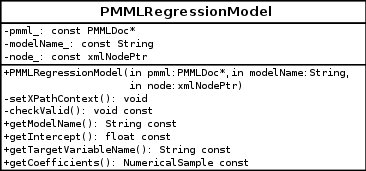
\includegraphics[scale=0.7]{PMMLRegressionModel.png}
    \caption{PMMLRegressionModel class}\label{fig:archi:PMMLRegressionModel}
  \end{center}
\end{figure}

The \texttt{PMMLRegressionModel} class is straightforward.  The \texttt{checkValid} private method ensures that
this regression model can be mapped to a \texttt{LinearLeastSquares} instance.  The following checks are performed:
\begin{itemize}
\setlength{\itemsep}{0pt}
\item \texttt{modelType} attribute, if present, must be equal to \texttt{linearRegression}
\item \texttt{functionName} attribute must be equal to \texttt{regression}
\item \texttt{normalizationMethod} attribute must be equal to \texttt{none}
\item there must be only one \texttt{RegressionTable} child element
\item this \texttt{RegressionTable} must contain only \texttt{NumericPredictor} children and not \texttt{CategoricalPredictor}
\item \texttt{exponent} attributes of \texttt{NumericPredictor} must be equal to 1
\end{itemize}

\subsubsection{PMMLNeuralNetwork}

\begin{figure}[htb]
  \begin{center}
    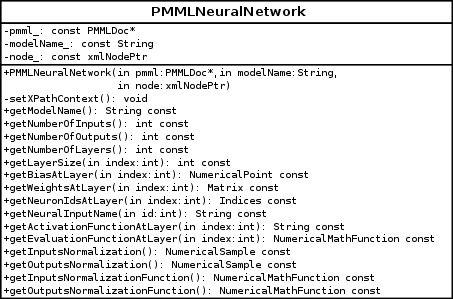
\includegraphics[scale=0.7]{PMMLNeuralNetwork.png}
    \caption{PMMLNeuralNetwork class}\label{fig:archi:PMMLNeuralNetwork}
  \end{center}
\end{figure}

The \texttt{PMMLNeuralNetwork} class parses XML data and provides accessor methods which are used by \texttt{NeuralNetwork}.
Most functions could be private, they are public only to help testing and debugging.

Any valid \texttt{NeuralNetwork} XML element should be supported.  There may be any number of hidden layers, neural layers may have any number of neurons, layers may be sparse, all known activation functions are supported.  The only restriction is with normalization of inputs and outputs, piecewise normalization is not supported.  This should not be a problem since Uranie stores PMML files with this format.

\paragraph{Note:}
\texttt{NumericalMathFunction} is built from string formulas.  In order to preserve accuracy, 20 digits are used.  The drawback is that pretty-printing looks uglier than with less digits.
